\documentclass[../../main.tex]{subfiles}
\begin{document}
This section will introduce the tests prompted by the requirements in section \ref{sec:Requirements} and present the results. These results will determine whether it has been possible to comply with the requirement specifications. Additional data from the tests can be seen in the digital appendix. 

To ease access to data from the FPGA during tests, a \textit{microblaze} has been implemented, which utilises UART to communicate directly with a computer. This allows for direct access to the position and velocity of the pan and tilt motor making data processing easier. 

\subsection{Microcontroller Timing Test}
Running multiple tasks on one microcontroller it is imperative to know, how much of the CPU time is utilised. If the CPU utilises too much time the risk of starvation is introduced, thus it is wanted to test whether the system can satisfy the requirement from section \ref{sec:Requirements}: 
\begin{itemize}
    \item The microcontroller is not to utilise more than 80\% of the total CPU time.
    \item It must be verified that the overhead does not compromise the timing of the system.
\end{itemize}

The test is executed with four controllers, the UART task, the SPI task and the UI task running with freeRTOS. The position controllers are scheduled at a frequency of \SI{200}{\hertz} and the velocity controllers at \SI{1000}{\hertz}. The timing of the tasks is done by driving pins high upon start and low finish of all individual tasks, thus enabling the possibility of timing the tasks with an oscilloscope.

\subsubsection*{Results}
Table \ref{tab:CPU_utilisation_test} shows the timing of running the controllers including the UART, SPI and UI task. Table \ref{tab:Task_Timing} shows the timing of the UART, SPI and UI respectively. 
Timing the duration of the tasks from the first task initiates to the last task terminates the duration of cycle is determined. T is the duration between the first cycle starts to the next cycle begins, as seen on figure \ref{fig:Schedueling_controllers}. This makes it possible to estimate the average duty cycle of the system:
\begin{equation}
    D_c=100-\left(\frac{T_{c1,avg}}{T_{avg}}\right)\cdot 100=100-\left(\frac{\SI{457,6}{\mu\second}}{\SI{992}{\mu\second}}\right)\cdot 100\approx 53,87\%
\end{equation}
where $T_{c1,avg}$ is the average duration of cycle 1 and $T_{avg}$ is the average time of T on figure \ref{fig:Schedueling_controllers}. 
\begin{table}[H]
\centering
\begin{tabular}{l|r|r|r|r|r|l}
& \textbf{1} & \textbf{2} & \textbf{3} & \textbf{4} & \textbf{5} & \multicolumn{1}{r}{\textbf{Unit}}                                  \\ \hline
Duration of cycle 1               & 458        & 456        & 456        & 460        & 458        & \SI{}{\mu\second} \\
T             & 990        & 988        & 994        & 994        & 994        & \SI{}{\mu\second} \\
Duty cycle                            & 53,73      & 53,85      & 54,12      & 53,72      & 53,92      & \%                   
\end{tabular}
\caption{Data regarding the duty cycle of the controller process scheduled with two position and two velocity controllers, the UART, SPI and UI task. The position controllers are scheduled at a rate of \SI{200}{\hertz} and the velocity controllers at \SI{1000}{\hertz}. Figure \ref{fig:Schedueling_controllers} illustrates the test.}
\label{tab:CPU_utilisation_test}
\end{table}

% Please add the following required packages to your document preamble:
% \usepackage{graphicx}
% Please add the following required packages to your document preamble:
% \usepackage{graphicx}
\begin{table}[H]
\centering
\begin{tabular}{l|c|r|r|r|r|r|l}
 & \multicolumn{1}{r|}{\textbf{Priority}} & \textbf{1} & \textbf{2} & \textbf{3} & \textbf{4} & \textbf{5} & \textbf{Unit}         \\ \hline
SPI\_transmit & 5                                      & 9,9        & 9,75       & 9,75       & 9,74       & 9,75       & \SI{}{\mu\second}                      \\
SPI\_receive  & 5                                      & 5,44       & 5,44       & 5,44       & 5,46       & 5,45       &   \SI{}{\mu\second}                    \\
UART          & 1                                      & 458        & 500        & 500        & 500        & 501        &  \SI{}{\mu\second}                     \\
UI            & 1                                      & NA         & NA         & NA         & NA         & NA         & \multicolumn{1}{c}{-}
\end{tabular}
\caption{Timing of SPI upon transmission and receiving, the UART task and UI, however the UI task was not able to be timed due to it being too quick.}
\label{tab:Task_Timing}
\end{table}

\begin{figure}
    \centering
    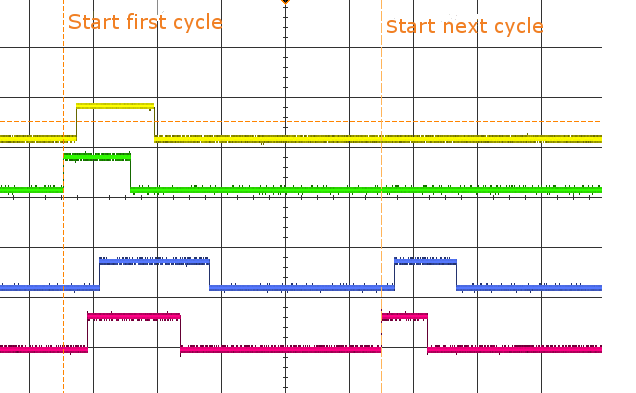
\includegraphics[width=0.7\textwidth]{Sections/Test/Images/Four_controllers_revised-white.png}
    \caption{Illustration of the scheduling of the four controllers running with two position and two velocity controllers, the UART, SPI and UI task. The yellow and the green are the position controllers run at a rate of \SI{200}{\hertz}. The blue and the red are the velocity controllers run at a rate of \SI{1000}{\hertz}.}
    \label{fig:Schedueling_controllers}
\end{figure}

However it is also possible to get an estimation of the overhead of the system by comparing the values of table \ref{tab:Single_Controller_test} and \ref{tab:CPU_utilisation_test}. An average overhead of approximately $\SI{42,6}{\mu\second}$ or \SI{5,7}{\percent} is calculated for the system.

\subsubsection*{Conclusion}
It has been possible to achieve an average CPU utilisation time of approximately \SI{ 53,87}{\percent}, thus satisfying the project stated requirement of a maximum CPU utilisation of \SI{80}{\percent}. Furthermore an average overhead is estimated to approximately $\SI{42,6}{\mu\second}$, hence not deemed to compromise the timing of the system.

\subsection{Processing time - Controllers}
It is wanted to examine the processing time of the controllers on the microcontroller. The requirement specification in section \ref{sec:Requirements} states:
\begin{itemize}
    \item All PID-controllers must be processed within a specified time frame to guarantee a minimum frequency. The minimum frequency and time period is to be determined.
\end{itemize}
To estimate a maximum allowed processing time for a controller, the CPU time is divided into five parts, four for the controllers and one for the remaining tasks. With a maximum CPU time utilisation of \SI{80}{\percent}, a single controller is to be processed within $\SI{160}{\mu\second}$.

Initially the microcontroller was tested with only one controller, namely velocity controller described in section \ref{sec:System_Integration_N_Implementation}. The parameters changed during the testing was, number of tabs on the derivative-term filter, without the filter and last only with a PI-controller. The test is carried out driving an output-pin high in the beginning of the controller task and low in the end, enabling the possibility of timing the task with an oscilloscope. The result of the test is seen in table \ref{tab:Single_Controller_test}.

\subsubsection*{Results}

As seen on table \ref{tab:Single_Controller_test} the PID-controller has an average processing time of $\SI{111,08}{\mu \second}$ with an 8th order derivative filter. In accordance with the requirement specification this is sufficient for a single controller. %It was however desired to test the influence of the derivative term and the additional filter on the derivative term. According to the test, the derivative term as implemented in the project adds an average of $\SI{16,68}{\mu\second}$ to the processing time.

\begin{table}[H]
\begin{tabular}{l|c|r|r|r|r|rl}
\textbf{Controller (Velocity)} & \multicolumn{1}{l|}{\textbf{Filter order}} & \textbf{1} & \textbf{2} & \textbf{3} & \textbf{4} & \multicolumn{1}{r|}{\textbf{5}} & \multicolumn{1}{r}{\textbf{Unit}}                                  \\ \hline
PID-controller                    & 4                                 & 104,4 & 104,4 & 104,6 & 104,6 & \multicolumn{1}{r|}{117,8} & \SI{}{\mu\second}      \\
\multicolumn{1}{c|}{-}  & 6                                 & 107,8 & 107,8 & 108   & 107,8 & \multicolumn{1}{r|}{108}   & \SI{}{\mu\second}        \\
\multicolumn{1}{c|}{-}            & 8                                 & 111,2 & 111   & 110,8 & 111,2 & \multicolumn{1}{r|}{111,2} & \SI{}{\mu\second}        \\
% PID without filter                & -                                 & 95,2  & 95,6  & 94,6  & 94,2  & \multicolumn{1}{r|}{95,2}  & \SI{}{\mu\second}        \\
% PI without D-term                 & -                                 & 94,4  & 94,4  & 94,6  & 94,2  & 94,4                       & \SI{}{\mu\second}     
\end{tabular}
\caption{Data regarding the duration of processing the position controller. The filter order is regarding the filter filtering the derivative term of the controller. All tests are made with a third order filter for the input.}
\label{tab:Single_Controller_test}
\end{table}
\subsubsection*{Conclusion}
A maximum allowed processing time for a single PID-controller is determined to be of $\SI{160}{\mu\second}$. Furthermore the processing time of a single PID-controller is tested with different parameters. A maximum processing time of $\SI{111,2}{\mu\second}$ is found, thus satisfying the requirement. 

\subsection{SPI Stress Test}
Using SPI as the only communication between the FPGA and the microcontroller, it is essential to test the reliability of the system to assure that no information is lost during transmission. 
\begin{itemize}
    \item Using SPI with a transmission frequency of \SI{2}{\kilo\hertz}, the FPGA is to receive 10000/10000 messages correct with no errors.
\end{itemize}
The test was preformed by sending 10000 messages from the microcontroller to the FPGA. Each message contains the value of a counter, starting at 0 and incrementing to 9999. Subsequent is each message transmitted to a computer with the help of the microblaze, and processed to check if all values are present and in the correct sequence.    
\begin{table}[H]
\centering
\begin{tabular}{c|c|c|c}
Test no. & Transmission Rate {[}kHz{]} & Msg. sent & Msg. received \\ \hline
1-5 & 2 & 10000 & 10000
\end{tabular}
\caption{Data regarding the five test performed with SPI.}
\label{tab:SPI-stresstest}
\end{table}

As seen in table \ref{tab:SPI-stresstest} the five test resulted in the same outcome, with all messages being received and in the correct sequence. 

\subsection{Test of Controller Designs}
%opdeling af afsnit
This section concerns the test of the PID-controllers using different methods for tuning and constellations. The parameters used in each test is shown in table \ref{tab:TestParameters}, and a deduced using the design requirements of \SI{5}{\percent} overshoot, \SI{1,5}{\second} settling time and \SI{0,5}{\second} rise time as described in section \ref{sec:System_Design}.
\begin{table}[H]
\centering
\begin{tabular}{c|c|c|c|c|c|c|c|c|}
      & \multicolumn{2}{l|}{Position Controllers} & \multicolumn{2}{l|}{Velocity Controller (tilt)} & \multicolumn{4}{c|}{Cascade Controller (tilt)}                                                                                                                                                                                \\ \hline
      & Tilt                & Pan                 & ZN                      & PP                    & \begin{tabular}[c]{@{}c@{}}ZN\\ Position\end{tabular} & \begin{tabular}[c]{@{}c@{}}ZN\\ Velocity\end{tabular} & \begin{tabular}[c]{@{}c@{}}PP\\ Position\end{tabular} & \begin{tabular}[c]{@{}c@{}}PP\\ Velocity\end{tabular} \\
$k_P$ & 9.450               & 4.920               & 0.519                   & 1.422                 & 8.740                                                 & 0.519                                                 & 7.528                                                 & 1.420                                                 \\ 
$k_I$ & 8.550               & 3.170               & 22.860                  & 7.800                 & 7.640                                                 & 22.860                                                & 7.589                                                 & 7.800                                                 \\ 
$k_D$ & 0.900               & 1.200               & 0.003                   & 0.065                 & 1.220                                                 & 0.003                                                 & 1.030                                                 & 0.065                                                 \\ 
\end{tabular}
\caption{Parameters used for each test. ZN is deduced using the Zielger-Nichols method and PP is deduced using pole placement.}
\label{tab:TestParameters}
\end{table}

%Test metoden
\subsubsection*{Single Position Controller using Pole Placement}

\begin{figure}[h]
     \centering
     \begin{subfigure}[b]{0.49\textwidth}
         \centering
         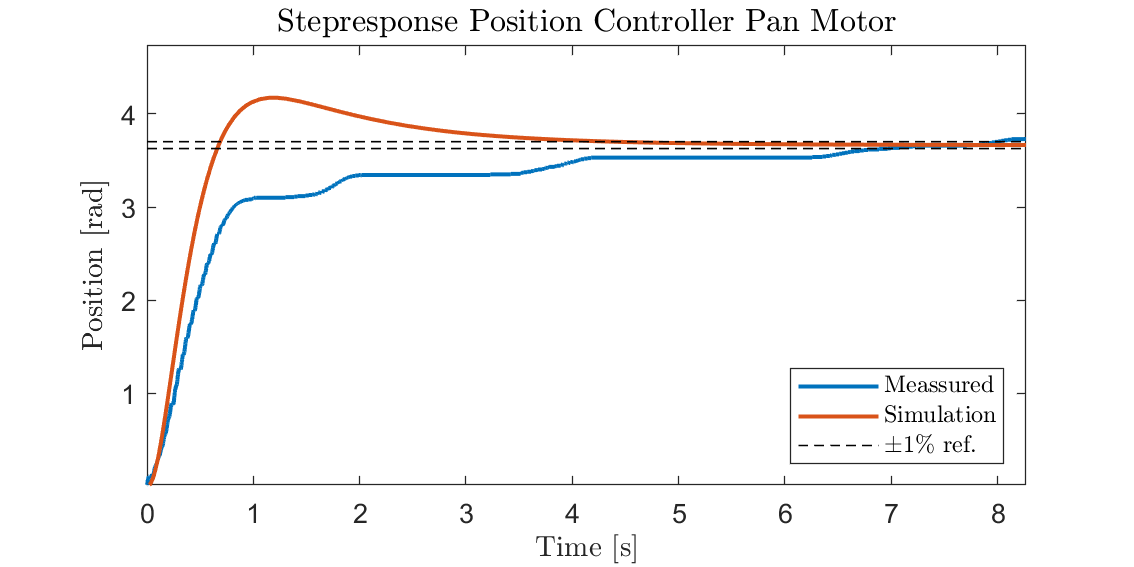
\includegraphics[width=\textwidth]{Sections/Test/Images/StepPanPosModel.png}
         \caption{Pan motor}
         \label{fig:StepPanPos}
     \end{subfigure}
     \hfill
     \begin{subfigure}[b]{0.49\textwidth}
         \centering
         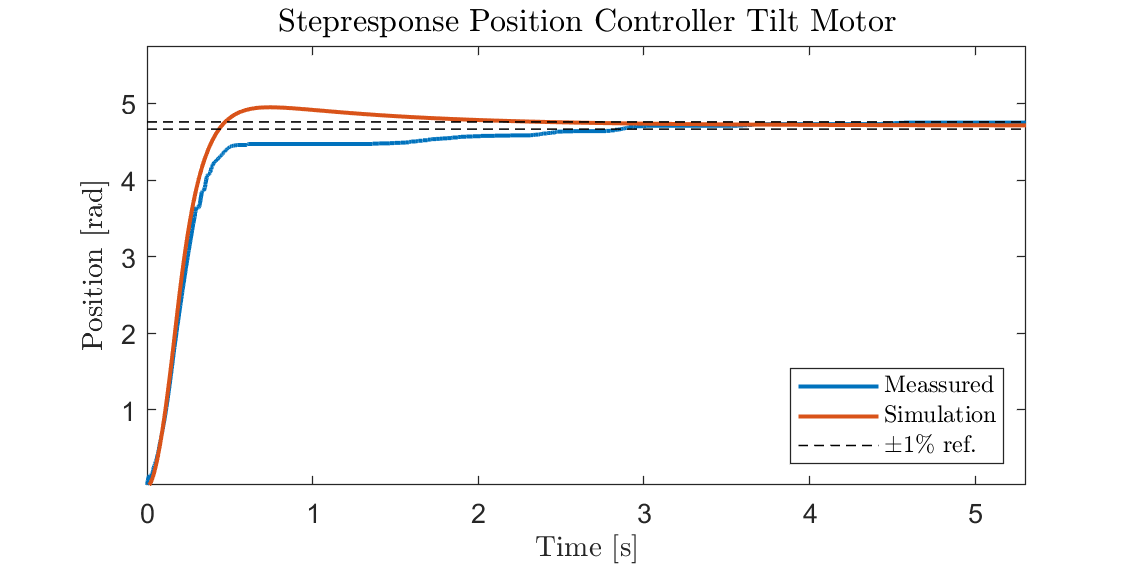
\includegraphics[width=\textwidth]{Sections/Test/Images/StepTiltPosModel.png}
         \caption{Tilt motor}
         \label{fig:StepTiltPos}
     \end{subfigure}
        \caption{Step response of the position using a single controller with pole placement. The measured response being an average of five tests.}
        \label{fig:singlePosController}
\end{figure}
The tests are executed with a reference point of $\theta = \frac{7\pi}{6}$ for the pan motor and $\theta = \frac{3\pi}{2}$. As seen on figure \ref{fig:StepPanPos} the measured response resembles the simulated response in the first part of the transition period. As there is stationary point in the measured response, it could look like that the pan has stopped moving for a bit properly due to friction in the physical setup. On figure \ref{fig:StepTiltPos} the measured response resembles the simulated quite well. The data for the tests can be seen on table \ref{tab:controller_data}. Applicable for both measurements is that they have no overshoot and longer settling times than the simulated. 


\subsubsection*{Velocity Controller for the Tilt Motor}
The velocity controller is tested using the Ziegler-Nichols and pole placement method on the tilt motor. A reference point of $\SI{20}{\mathrm{rad}/\second}$ is used. As seen on figure \ref{fig:StepVelZN} the measured response initially resembles the simulated signal using the Ziegler-Nichols method. Seen on figure \ref{fig:StepVelModel}, using pole placement a very slow response compared to the simulated is achieved. The reason for this behaviour is discussed in section \ref{sec:Discussion}. Applicable for both tests are that the measured signal oscillates to a point, where it never settles. Data regarding the performance of the controller is seen in table \ref{tab:controller_data}.

\begin{figure}[h]
     \centering
     \begin{subfigure}[b]{0.49\textwidth}
         \centering
         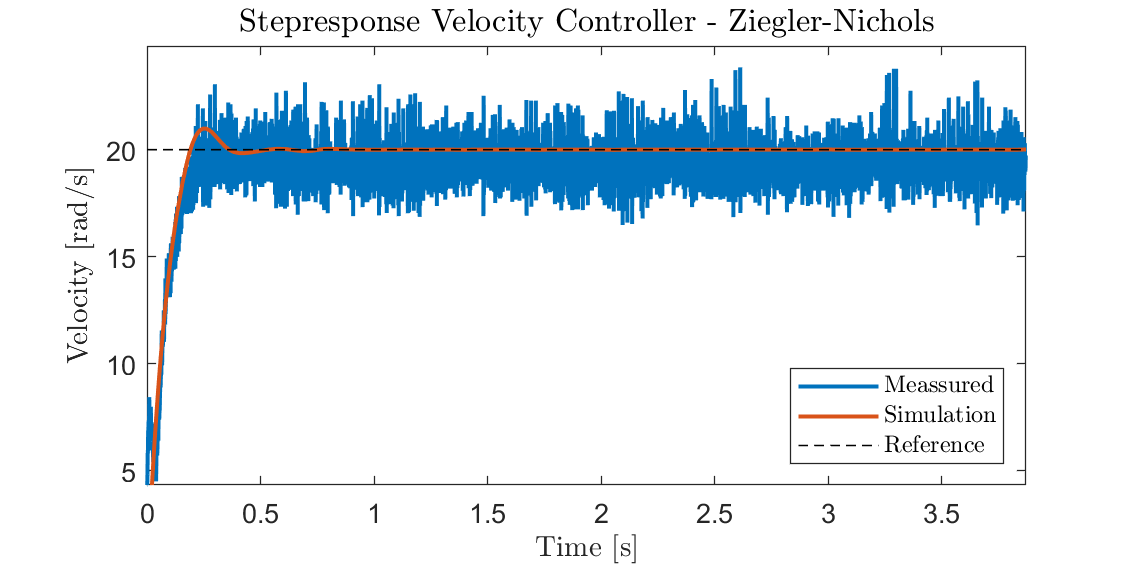
\includegraphics[width=\textwidth]{Sections/Test/Images/StepVelocityZN.png}
         \caption{Ziegler-Nichols}
         \label{fig:StepVelZN}
     \end{subfigure}
     \hfill
     \begin{subfigure}[b]{0.49\textwidth}
         \centering
         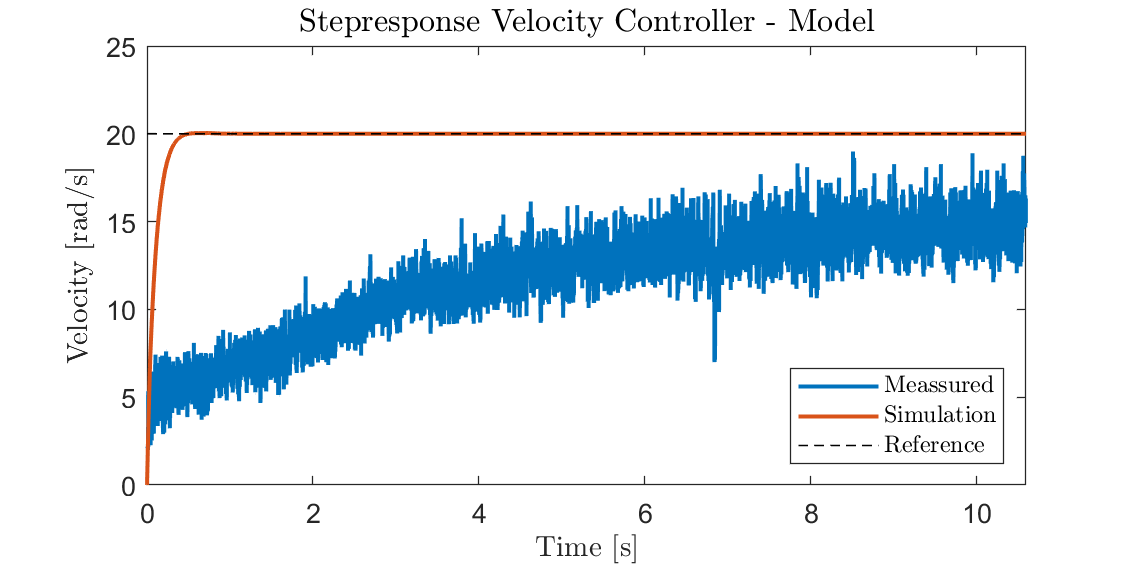
\includegraphics[width=\textwidth]{Sections/Test/Images/StepVelocityModel.png}
         \caption{Pole Placement}
         \label{fig:StepVelModel}
     \end{subfigure}
        \caption{Step response of a single velocity controller on the tilt motor. The measured response being an average of five tests.}
        \label{fig:VelocityTilt}
\end{figure}

\subsubsection*{Cascade Position Controller for the Tilt Motor}
The cascaded PID-controller design is tested on the tilt motor using the Ziegler-Nichols and pole placement method with a reference point of $\theta = \frac{3\pi}{2}$. Figure \ref{fig:Cascade_ZN_tilt} shows that using the Ziegler-Nichols method, the measured signal resembles the simulated response quite well. However using the pole placement method, illustrated on figure \ref{fig:cascade_model_tilt}, the measured response has a lot more overshoot than the simulated. The results can be seen in table \ref{tab:controller_data}.

\begin{figure}[h]
     \centering
     \begin{subfigure}[b]{0.49\textwidth}
         \centering
         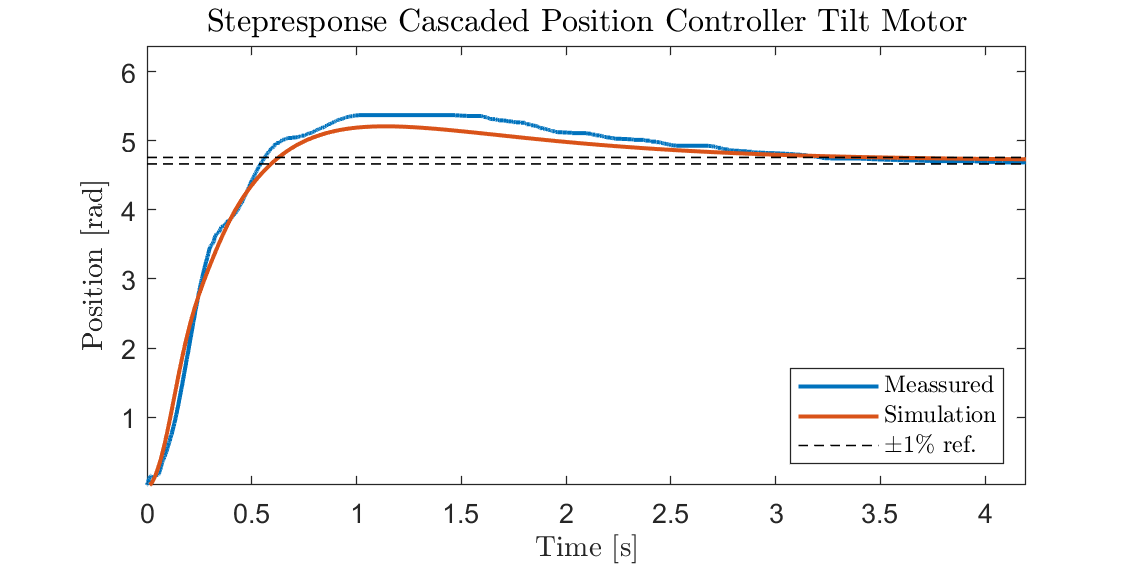
\includegraphics[width=\textwidth]{Sections/Test/Images/cascade_ZN_tilt.png}
         \caption{Ziegler-Nichols method}
         \label{fig:Cascade_ZN_tilt}
     \end{subfigure}
     \hfill
     \begin{subfigure}[b]{0.49\textwidth}
         \centering
         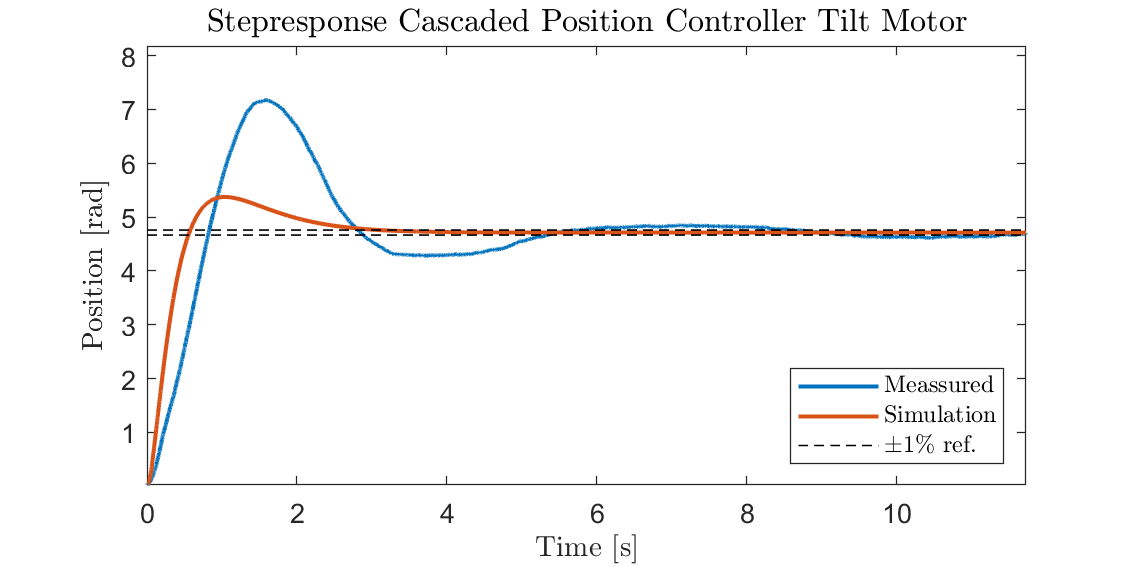
\includegraphics[width=\textwidth]{Sections/Test/Images/cascade_Model_tilt.png}
         \caption{Pole Placement method}
         \label{fig:cascade_model_tilt}
     \end{subfigure}
        \caption{Step response of a cascaded PID-controller for the position of the tilt motor. The measured response being an average of five tests.}
        \label{fig:CascadeTilt}
\end{figure}

\subsubsection*{Cascade Position Controller for the Pan Motor}
The cascaded controller on the pan motor is executed using a reference point of $\theta = \frac{7\pi}{6}$. The parameters are identical with the ones used for the cascaded tilt controller. According to figure \ref{fig:cascade_ZN_pan}, the measured signal seems to have a slower response than the simulated. However neither the simulated nor the measured response are considered ideal, which is discussed further in section \ref{sec:Discussion}.

\begin{figure}[h]
    \centering
    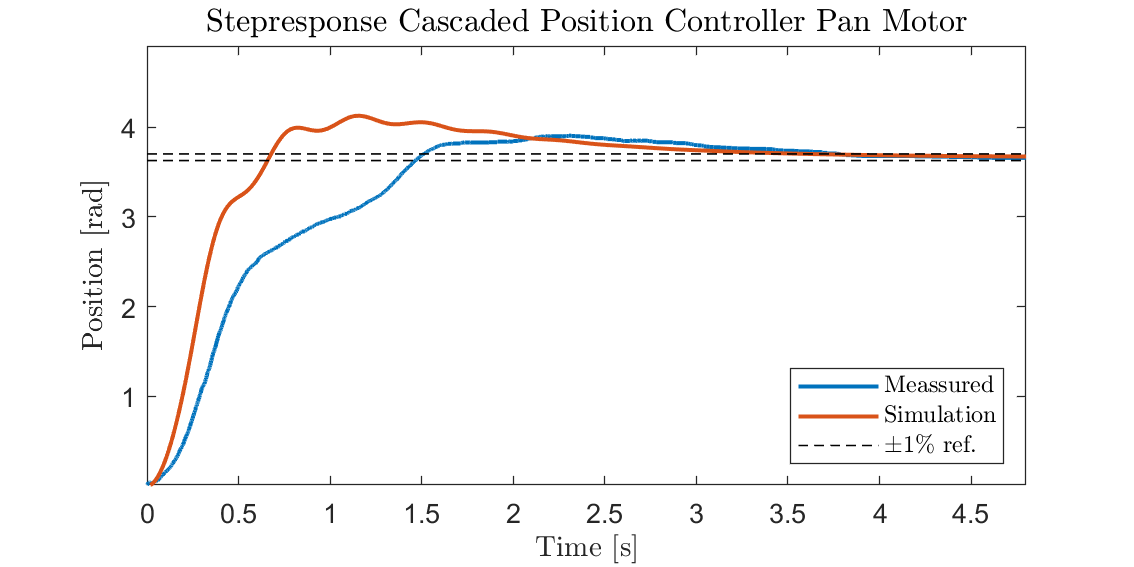
\includegraphics[width = 0.7 \textwidth]{Sections/Test/Images/cascade_ZN_pan.png}
    \caption{Position step response using a cascaded PID-controller for the pan motor. The measured response being an average of five tests.}
    \label{fig:cascade_ZN_pan}
\end{figure}

\subsubsection*{Results}
Table \ref{tab:controller_data} shows the data regarding the performance of the different PID-controllers. As it is seen none of the designed controllers satisfies the specifications of less than \SI{5}{\percent} overshoot, \SI{1,5}{\second} settling time and \SI{0,5}{\second} rise time, however some controllers achieved better results than others. The single position PID controller seems to have the overall best performance in relation the the requirement specifications. The reason for the deviations comparing the simulation and the measured are discussed in section \ref{sec:Discussion}.
\begin{table}[H]
    \centering
    \begin{tabular}{c|c|c|c|c|c}
         Controller & Motor & Method & Overshoot (\%) & Settling Time (s)  & Rise Time (s) \\ \hline
         Position & Pan & Pole placement & 14.3 & 8.27 & 1.74  \\
         Position & Tilt & Pole placement & 0.8 & 2.86 & 0.34  \\
         Velocity & Tilt & Ziegler-Nichols & 19.2 & N/A & 0.15  \\
         Velocity &Tilt & Pole placement & N/A & N/A & 7.8 \\
         Cascade & Tilt  & Pole placement & 52 & 11.47 & 0.61 \\
         Cascade & Tilt & Ziegler-Nichols & 14 & 3.22 & 0.38  \\
         Cascade & Pan & Ziegler-Nichols & 6.6 & 3.78 & 1.13  \\
         
    \end{tabular}
    \caption{Step response specifications of the different controllers tested. Entries marked with N/A could not be determined from the available data.}
    \label{tab:controller_data}
\end{table}

\end{document}